\documentclass{article}

\usepackage{import}
\usepackage{graphicx}
\usepackage{subfig}
\usepackage[margin = 1in]{geometry}
\usepackage{amsmath}


\begin{document}

\section*{to do list}

\begin{itemize}
	\item plot to justify linear trend, show spurious correlation
	\item outline
	\begin{enumerate}
		\item intro
		\item Theory
		\begin{enumerate}
			\item Romer production function: introduce knowledge spillover, both theoretically interesting and a simple way to introduce increasing returns to R\&D. Explain K and k.
			\item representative firm of supply chain: note an unproven theorem that the size of the externality decreases in retailer productivity.
			\item Comparing Subsidization of Demand, Installers, and Suppliers: can say demand vs retailer subsidy hold by similar argument to demand vs supplier.
		\end{enumerate}
		\item How Do Installers Modulate the Affect of Demand Subsidies?
		\begin{enumerate}
			\item data
			\item comparative static
			\item productivity regression
			\item subsidy regression
			\end{enumerate}
		\item conclusion
	\end{enumerate}
\end{itemize}

\section{intro}

\section{Preliminary Analysis}

\begin{equation}
log(y_i) = \alpha + \beta ~ log(subsidy_i) + \vec{\gamma} ~ \vec{month} + \vec{eta} ~ \vec{year} + \delta~ t + \epsilon
\end{equation}

\begin{table}
\begin{center}
Aggregate Installer Productivity Per Month By IOU

\vspace{0.5cm}

A. Total Size (DC, Kw) of Systems Installed Per Month, 

Per Total Size Committed to Per Month, By IOU

\vspace{0.25cm}

\subimport{../term_paper_analysis/}{size_comp_res}

\vspace{0.5cm}

B. Quantity Installed Per Month, 

Per Quantity Committed to Per Month, by IOU

\vspace{0.25cm}

\subimport{../term_paper_analysis/}{q_comp_res}
\end{center}
\caption{test}
\label{agg_prod_tab}
\end{table}


\begin{figure}
\begin{center}
Aggregate Installer Productivity Per Month By IOU
\begin{tabular}{cc}
\subfloat[Quantity installed in PGE]{\includegraphics[width = 3in]{q_comp_PGE}} &
\subfloat[Total size installed in PGE]{\includegraphics[width = 3in]{size_comp_PGE}}\\
\subfloat[Quantity installed in SCE]{\includegraphics[width = 3in]{q_comp_SCE}} &
\subfloat[Total size installed in SCE]{\includegraphics[width = 3in]{size_comp_SCE}}\\
\subfloat[Quantity installed in SDGE]{\includegraphics[width = 3in]{q_comp_SDGE}} &
\subfloat[Total size installed in SDGE ]{\includegraphics[width = 3in]{size_comp_SDGE}}\\
\end{tabular}
\end{center}
\caption{The y-axis is the sum of the total system size or equipment installed by installers in a month in an IOU. The x-axis is the sum of the total system size or equipment that installers were committed to installing during that month, according to subsidy applications. For example, If an installers in an IOU installed 40 Kw of system in July 2010, and were named on subsidy applications for projects totaling another 60 Kw in system size in that IOU during July 2010, then the observation for that IOU-month-year has 40 Kw installed, and 100 Kw committed to. Note this means that installed projects are counted as commitments. Axes are scaled symmetrically and identically so as to fit all data and allow comparison. The blue points are IOU-month-year observations. The red line is the best linear fit.}
\label{agg_prod_fig}
\end{figure}

\begin{table}
\begin{center}
Effect of Subsidy on Solar Industry Output

\vspace{0.5cm}

A. Effect on Total Size (DC, Kw) of Subsidy (\$/Watt), by IOU

\vspace{0.25cm}

\begin{tabular}{llll}
\hline
               & PGE      & SDGE     & SCE       \\
\hline
log\_subsidy   & 0.0922   & 0.2246   & -0.3465   \\
               & (0.0247) & (0.1315) & (0.0213)  \\
R-squared      & 0.0087   & 0.0330   & 0.0838    \\
R-squared Adj. & 0.0082   & 0.0259   & 0.0832    \\
N              & 56037    & 2604     & 34270   
\\ \hline
Month Fixed Effects & Yes & Yes & Yes \\ 
Year Fixed Effects & Yes & Yes & Yes \\
Month Time Trend & Yes & Yes & Yes \\ \hline
Installer Productivity (Size) & 0.1766 & 0.9643 & 0.1850 \\ \hline
\end{tabular}

\vspace{0.5cm}

B. Effect on Quantity Installed of Subsidy (\$/Watt),, by IOU

\vspace{0.25cm}

\begin{tabular}{llll}
\hline
               & PGE      & SDGE     & SCE       \\
\hline
log\_subsidy   & -0.0657  & 0.2826   & 0.0274    \\
               & (0.0272) & (0.1344) & (0.0115)  \\
R-squared      & 0.0122   & 0.0214   & 0.0127    \\
R-squared Adj. & 0.0119   & 0.0146   & 0.0121    \\
N              & 56037    & 2604     & 34270   
\\ \hline
Month Fixed Effects & Yes & Yes & Yes \\ 
Year Fixed Effects & Yes & Yes & Yes \\
Month Time Trend & Yes & Yes & Yes \\ \hline
Installer Productivity (Quantity) & 0.2131 & 0.9621 & 0.2452 \\ \hline
\end{tabular}

\end{center}
\caption{Regression takes place using individual CSI subsidy applications as observations. Outcome of interest is either the logarithm of total size of system installed, or the logarithm of total quantity of generators and inverters installed. The independent variable of interest is the logarithm of the subsidy. Subsidy is $\$/Watt$. The estimated productivity of installers is included in the last line of each table. IOUs with higher productivity have a higher correlation between demand and subsidy level.}
\label{subsidy_table}
\end{table}

\begin{figure}
\begin{center}
Monthly Subsidy Level and Histogram of All Application Reception Dates


\begin{tabular}{c}
\subfloat[PGE]{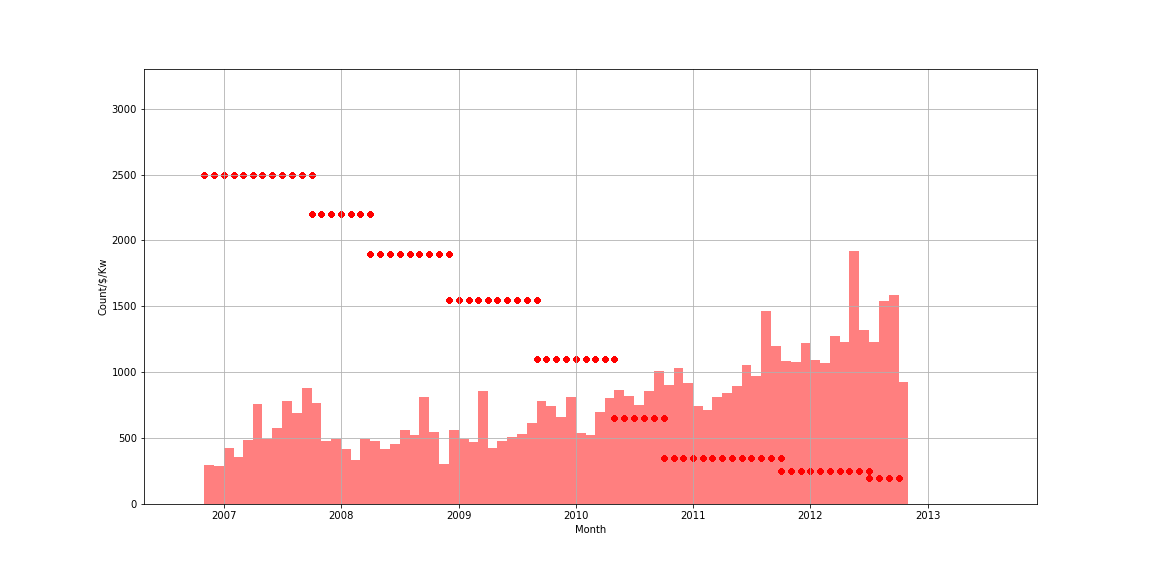
\includegraphics[width = 5in]{app_hist_pge}}\\
\subfloat[SCE]{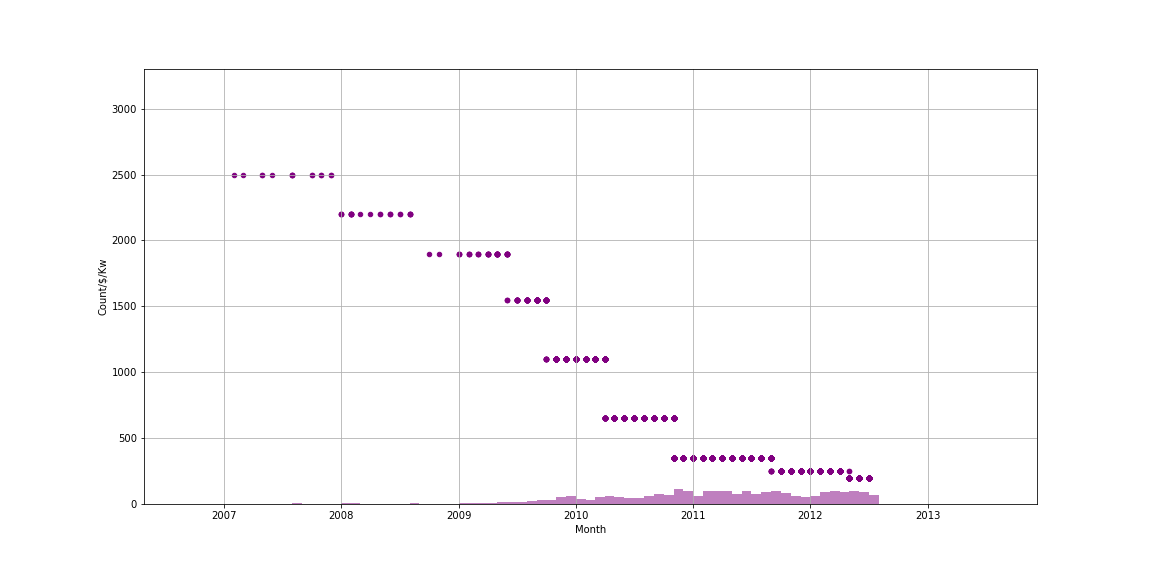
\includegraphics[width = 5in]{app_hist_sdge}}\\
\subfloat[SDGE ]{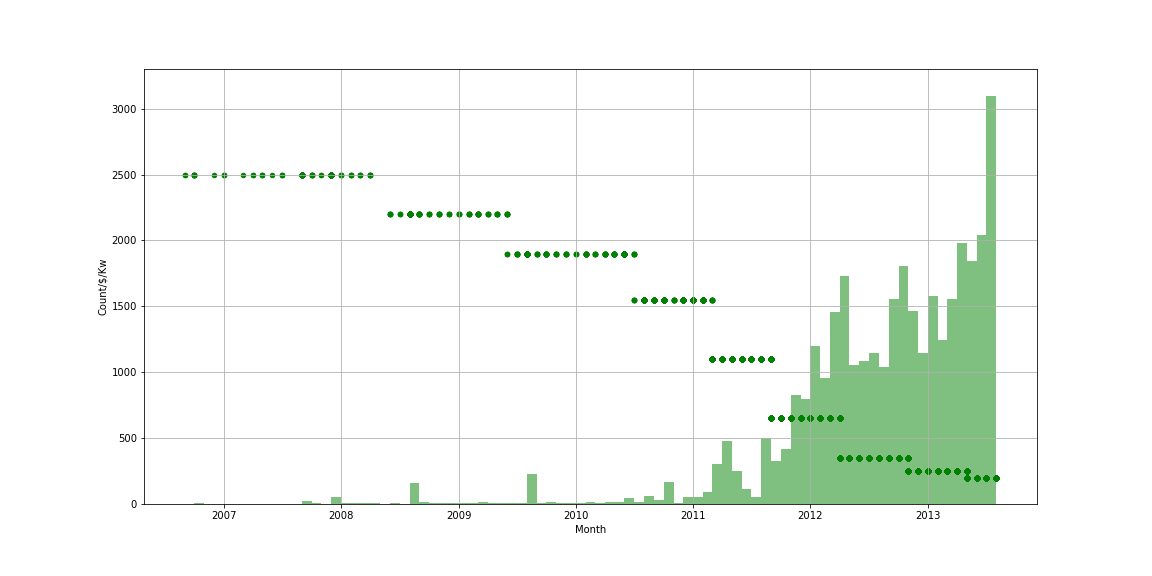
\includegraphics[width = 5in]{app_hist_sce}}\\
\end{tabular}

\end{center}
\caption{The bars are counts of applications received within a month. The dots are subsidy levels during month when applications were received.}
\end{figure}

\end{document}